\subsection{Creating a Multi-Language Environment}
A verification environment typically consists of a system UVC containing
multiple subsystem UVCs, interface UVCs or module UVCs. These are composed in a
hierarchical way. With UVM-ML an environment can be constructed with components,
which are implemented in different frameworks. For example it could be composed
of an interface UVC implemented in UVM-SV and a module UVC in
UVM-\textit{e}. \\
When planing to create such a multi-language environment, there
are two possible approaches supported by UVM-ML to achieve this goal. Firstly an
\emph{unified hierarchy} can be created or alternatively a \emph{side-by-side}
environment. In an \emph{unified hierarchy} a child component implemented in one
verification language is instantiated from a parent component in another
verification language. In contrast, when creating a \emph{side-by-side} architecture,
the environment contains multiple tops.

\subsubsection{Creating an \emph{Unified Hierarchy} Environment}
To implement an \emph{unified hierarchy} each component which instantiates a
component of another framework needs to create and connect a proxy to
this component (this can be seen in figure~\ref{fig:UVM_ML_unified}). Then the
backplane applies operations which are performed on the proxy to the
corresponding component in the other verification language. This gives the
opportunity to use some of benefits of UVM-ML. It is possible to use a predefined
phasing in this environment, where phases like \lstinline$build$, \lstinline$connect$ or \lstinline$run$ are
performed depth-first. This ensures that dependencies between the components of
different frameworks are resolved in the right way \cite{uvm_ml_ref}. Also sub-components can be
configured which increases the reusability of the environment. When the
environment is included in some other environment, only the top component needs
to be configured and all sub-components are configured automatically. As a result of
this, it is recommended to implement such an environment \cite{uvm_ml_user}.\\
Following it is described how to create a \emph{unified hierarchy} which
instantiates an UVM-SV component within an UVM-\textit{e} unit and vice versa.

\begin{figure}[htb]
 \centering
 %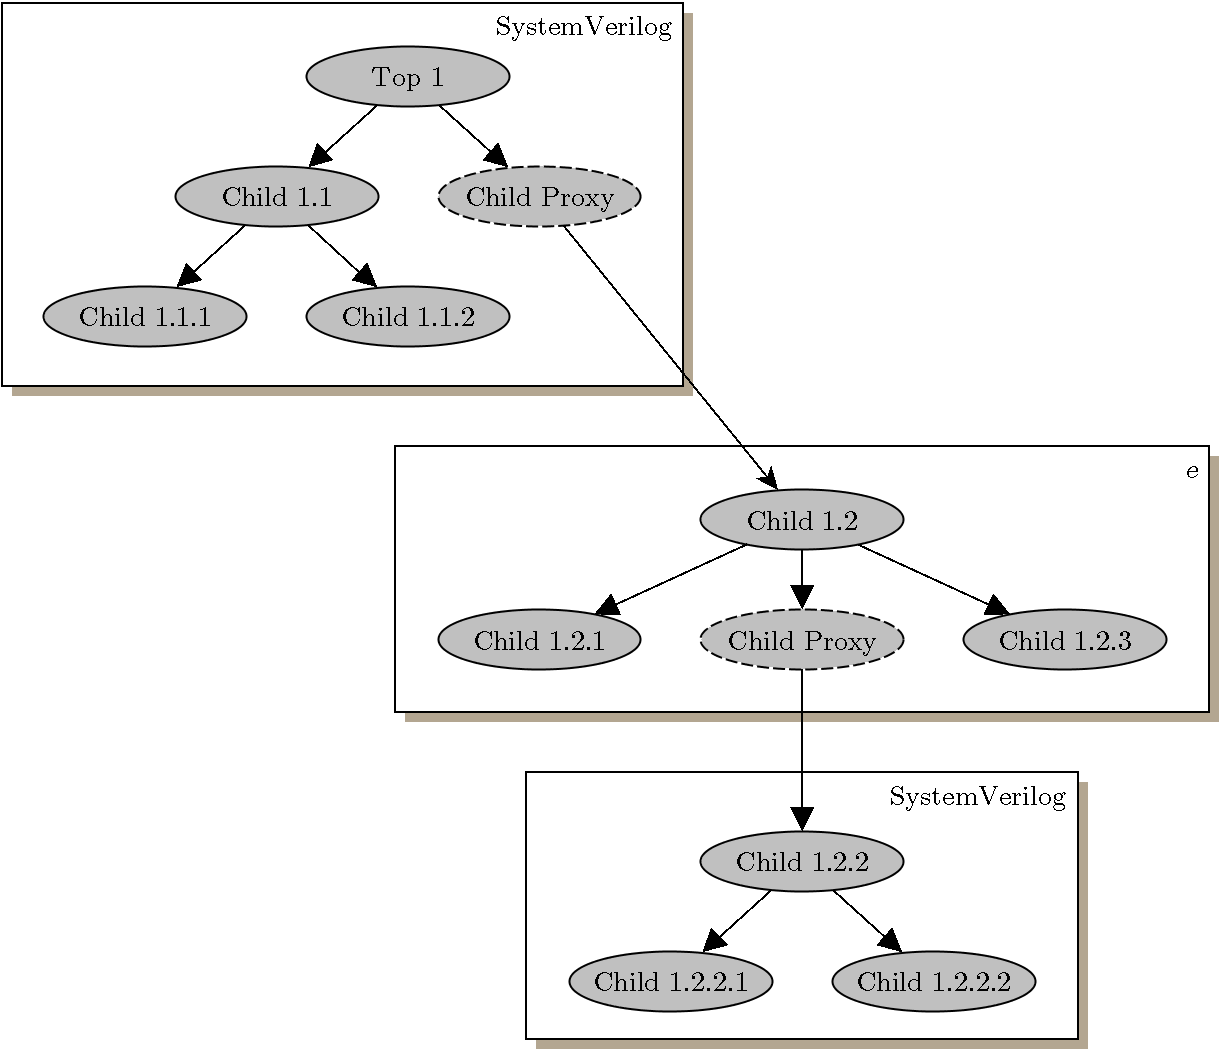
\includegraphics[width=1.0\textwidth,angle=0]{abb/UVM_ML_unified}
 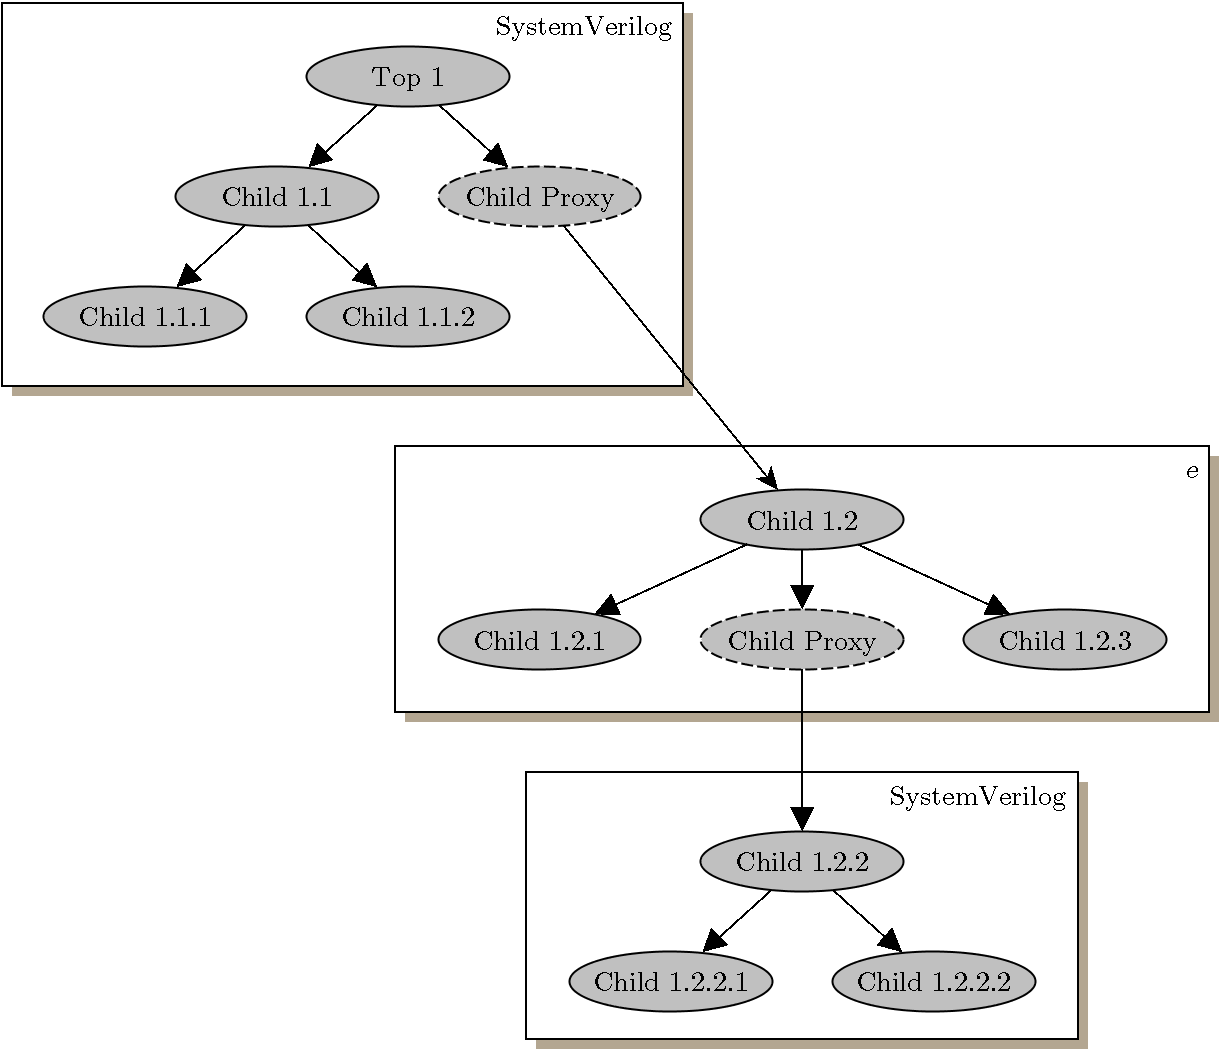
\includegraphics[scale=0.3]{abb/UVM_ML_unified}
 \caption{Structure of an \emph{unified hierarchy} environment}
\label{fig:UVM_ML_unified}
\end{figure}

\paragraph{Instantiating an UVM-SV Component within an UVM-\textit{e} Unit}
\label{sv_inside_e}
When instantiating an UVM-SV component within an UVM-\textit{e} unit,
it is necessary to instantiate a proxy unit inside the UVM-\textit{e} unit. After that the
proxy unit and the UVM-SV component need to be connected. \\
An example for the code of the extended UVM-SV component can be seen in
example~\ref{lst:SV_unified_sub}.
It is recommended to extend the UVM-SV component
(line~\ref{line_extend_component}), which will
be reused. After that, all multi-language functionalities are put inside this new
component. This ensure, that the original component can still be used in
non-multi-language environments. For this purpose the single-language UVC is imported (line~\ref{line_uvm_uvc_package}) and everything is put inside of a package for the multi-language functionalities (line~\ref{line_uvm_uvc_ml_package}). This package needs to include the UVM
package (line~\ref{line_uvm_package}/\ref{line_uvm_macros}) as well as the adapter
package for UVM-SV (line~\ref{line_uvm_ml_package}).
After that all additional multi-language functionalities can be put inside the
class like configuring the sub-component (see section~\ref{ml_config}) or data
communication via TLM interfaces (see section~\ref{ml_tlm}).
\medskip
\lstset{language={SystemVerilog}, numbers=left, escapechar=|}
\begin{lstlisting}[frame=htrbl, caption={SystemVerilog: extended multi-language component}, label={lst:SV_unified_sub}]
package ml_uvc_pkg;					|\label{line_uvm_uvc_ml_package}|

import uvm_pkg::*;					|\label{line_uvm_package}|
`include "uvm_macros.svh"			|\label{line_uvm_macros}|
import uvm_ml::*;					|\label{line_uvm_ml_package}|
import uvc_pkg;						|\label{line_uvm_uvc_package}|

class ml_uvc_env extends uvc_env;			|\label{line_extend_component}|
  `uvm_component_utils(ml_uvc_env)
  function void build_phase(uvm_phase phase);
    // Additional multi-language functionalities
    // introduced in the next subsections
  endfunction : build_phase
endclass : ml_uvc_env

endpackage : ml_uvc_pkg;
\end{lstlisting}
\medskip
Corresponding to the extensions in the UVM-SV component the UVM-\textit{e}
unit needs to include a proxy unit for the foreign component (see example~\ref{lst:e_unified_top}).
This can be done by instantiating an unit of type
\lstinline$child_component_proxy$ (line~\ref{line_uvm_ml_e_proxy}) which is a
predefined data type in the UVM-\textit{e} adapter.
Through constraining the proxy unit's \lstinline$type_name$ field
(line~\ref{line_uvm_ml_e_proxy_keep}) the
SystemVerilog component is integrated into the hierarchy. Thereby the string
needs to be composed of \lstinline$target_frmw_indicator:component_type_name$. Firstly
\lstinline$target_frmw_indicator$ (case-insensitive) identifies the framework
of the instantiated foreign child component and can be \lstinline$SV$ for
UVM-SV, \lstinline$e$ for UVM-\textit{e} or \lstinline$SC$ for UVM-SystemC. Followed by
\lstinline$component_type_name$, which is the type of the instantiated component.
\medskip
\lstset{language=e, numbers=left, escapechar=|}
\begin{lstlisting}[frame=htrbl, caption={\textit{e}: instantiating the UVM-SV component in the UVM-\textit{e} unit},
label={lst:e_unified_top}]
unit e_uvc_env {
  sv_uvc: child_component_proxy is instance;	|\label{line_uvm_ml_e_proxy}|
    keep sv_uvc.type_name == "SV:ml_uvc_env";|\label{line_uvm_ml_e_proxy_keep}| 
};
\end{lstlisting}

\paragraph{Instantiating an UVM-\textit{e} Unit Within an UVM-SV Component}
When reusing an UVM-\textit{e} unit inside of an UVM-SV component it is
necessary to integrate a proxy for the e unit within the UVM-SV
component. After that, the proxy and foreign component are connected.\\
As shown in example~\ref{lst:SV_unified_top} this proxy component is created by
declaring a component of type \lstinline$uvm_component$ inside of the parent
component (line~\ref{line_sv_declare_proxy}). In the \lstinline$build_phase$ this proxy component is
instantiated via calling \lstinline$uvm_ml_create_component$ (line~\ref{line_sv_create_proxy}) with the following
syntax:
\medskip
\lstset{language={}, numbers=none, escapechar=|}
\begin{lstlisting}
function uvm_ml::child_component_proxy uvm_ml_create_component(
  string target_frmw_indicator,
  string component_type_name,
  string instance_name,
  uvm_component parent=null)
\end{lstlisting} 
\medskip
Where \lstinline$target_frmw_indicator$ indicates the framework adapter of the
foreign component (see section~\ref{sv_inside_e}). Secondly
\lstinline$component_type_name$ is the type of the foreign component according
to its declaration inside its framework. After that, \lstinline$instance_name$ is the name
of the instance of the component proxy. Finally \lstinline$parent$ is the handle of
the parent instance (\lstinline$this$ indicates the current component).\\
Multi-language functionalities are already integrated in UVM-\textit{e}. Bacause of this, the child unit does not need any changes
to support the creation of an \emph{unified hierarchy} environment.
\medskip
\lstset{language=SystemVerilog, numbers = left, escapechar=|, breaklines=true}
\begin{lstlisting}[frame=htrbl, caption={SystemVerilog: instantiating an e unit}, label={lst:SV_unified_top}]
import uvm_ml::*;

class testbench extends uvm_env;
  uvm_component e_uvc;|\label{line_sv_declare_proxy}|
  `uvm_component_utils(testbench)

  function void build_phase(uvm_phase phase);
    super.build_phase(phase);
    e_uvc = uvm_ml_create_component("e", "uvc_env_u", "e_uvc", this); |\label{line_sv_create_proxy}|
  endfunction
endclass : testbench
\end{lstlisting}

\subsubsection{Creating a \emph{Side-by-Side} Environment}

When there is no need to create an \emph{unified hierarchy} environment, UVM-ML supports also the ability to build an
environment with multiple tops as displayed in figure~\ref{fig:UVM_ML_side_by_side}. Here each tree inside of a
framework has its root instantiated as top component. This architecture is called \emph{side-by-side} and best
applicable when there is only limited synchronization required between the components of different frameworks. This is
indicated by the limitations of the architecture. It is not possible to use multi-language configuration as described in
section~\ref{ml_config}. Additionally the behavior of the phase execution is limited. Here each phase is first executed
completely on one tree before moving on to the next one. 

\begin{figure}[htb]
 \centering
 %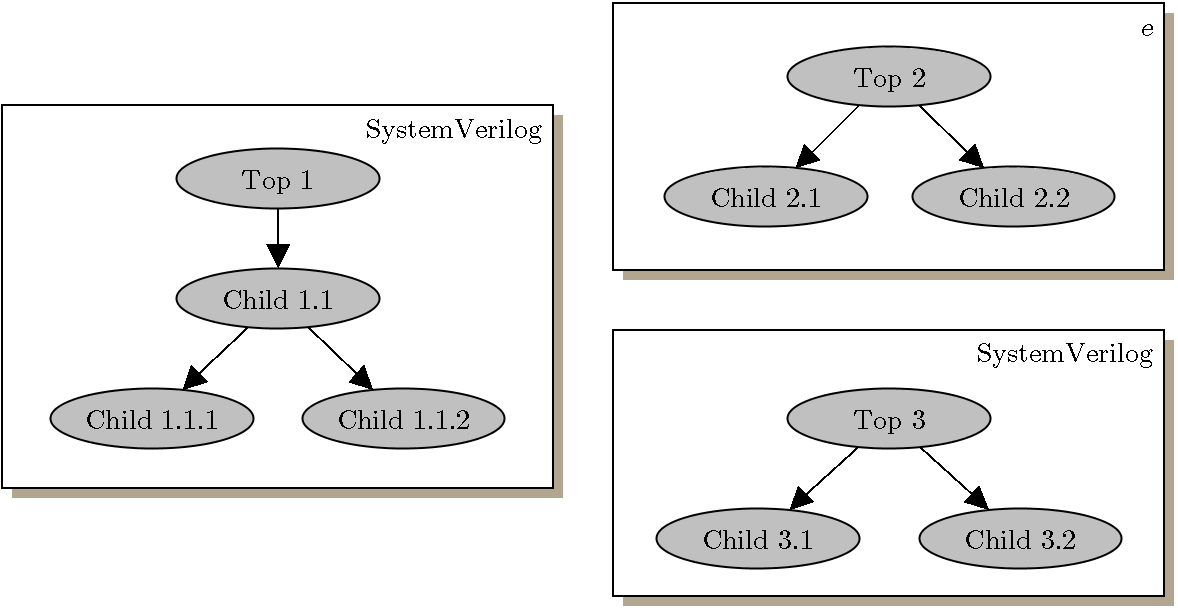
\includegraphics[width=1.0\textwidth,angle=0]{abb/UVM_ML_side_by_side}
 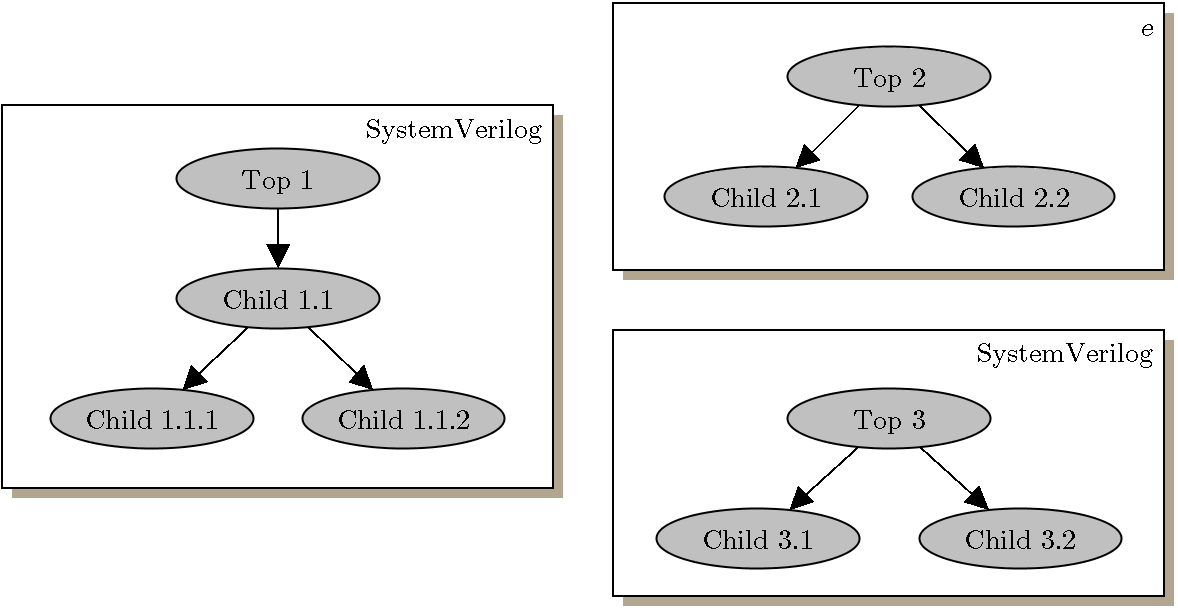
\includegraphics[scale=0.3]{abb/UVM_ML_side_by_side}
 \caption{Structure of a \emph{side-by-side} environment}
\label{fig:UVM_ML_side_by_side}
\end{figure}